\documentclass{article}
\usepackage{graphicx}
\usepackage{amssymb}
\usepackage{amsmath}
\usepackage{eurosym}
\usepackage{fullpage}
\usepackage{multirow}
\usepackage{fancyhdr}
\usepackage{amsmath}
\pagestyle{empty}
\usepackage{placeins}
\usepackage{changepage}
\usepackage[dvipsnames]{xcolor}
\usepackage{collectbox}
\usepackage{wrapfig}
\usepackage[utf8]{inputenc}
\usepackage[english]{babel}
\usepackage{gensymb}
\usepackage{tikz}
\usepackage{pgfplots}
\usepackage{graphicx}
\usepackage{booktabs}
\usepackage{enumitem}
\usepackage{afterpage}
\usepackage{overpic}
\usetikzlibrary{calc}
\usetikzlibrary{calc,patterns,angles,quotes}
\usepackage{xfrac}
\usetikzlibrary{automata, positioning}
\usepackage{color,soul}


\pgfplotsset{width=9cm,height=6.5cm,compat=1.9}

\setcounter{page}{1}


% Alternate method of doing solution function.
%\newcommand{\sol}[1]{}
%\renewcommand{\sol}[1]{{\color{blue} #1 \fi}}

%----------------------------------COMMANDS----------------------------------------------------
%---Create function to control text solution display----------------%
\newif\ifPrintSolution
\newcommand{\showSolution}{\PrintSolutiontrue}
\newcommand{\sol}[1]{\ifPrintSolution {\color{blue} #1 } \fi}
%---END Solution Function-------------------------------------------%

%---Create function to control R-Code solution display--------------%
\newcommand{\solR}[1]{} 
%---END R-Code Solution Function------------------------------------%

%%%%%%%%%%% Turn ON/OFF text solutions with this command%%%%%%%%%%%
\showSolution % comment out to hide solutions 
%%%%%%%%%%% Turn ON/OFF R-code solutions with this command%%%%%%%%%
\renewcommand{\solR}[0]{} % Comment out to hide R-Code Solutions

%------------------------------------------------------------------------------------------------

% Use \sol for text solutions and \solR for code chunk solutions

\begin{document}


\noindent \textbf{MA206 Lesson 1 - Introduction to Statistical Analysis}
\vspace{.1in}

\textbf{Understand the 6-Step Process}

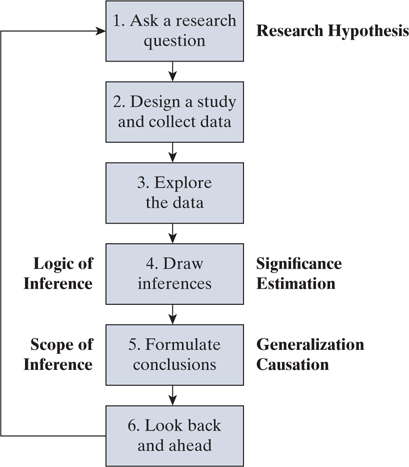
\includegraphics[scale=0.6]{6_Step_Process.png}

\vspace{0.25in}

\textbf{Understand the 4 Pillars of Statistical Inference}\\

\hspace{0.1in} \textbf{Significance}

\vfill
\sol{How \textbf{Strong} is the evidence of an effect?}

\hspace{0.1in} \textbf{Estimation}

\vfill
\sol{What is the \textbf{size} of the effect?}

\hspace{0.1in} \textbf{Generalization}

\vfill
\sol{How \textbf{broadly} do the conclusions apply?}

\hspace{0.1in} \textbf{Causation}

\vfill
\sol{Can we say what \textbf{caused} the observed difference?}


\vspace{0.2in}
\textbf{Understand the following terminology}

\hspace{0.1in} \textbf{Observational Units}

\vfill
\sol{These individual entities on which data are recorded}

\hspace{0.1in} \textbf{Categorical Variable}

\vfill
\sol{Variables with non-numeric values or with which arithmetic cannot be done}

\hspace{0.1in} \textbf{Quantitative Variable}

\vfill
\sol{Variables with numeric values with which arithmetic can be done}

\hspace{0.1in} \textbf{Distribution}

\vfill
\sol{The pattern of outcomes of a variable}

\pagebreak

\textbf{1) } \hspace{0.1in} When surveys are administered, it is hoped that the respondents give accurate answers. Does the mode of survey delivery affect this? American researchers investigated this question (Schober et al., 2015). They had 634 people agree to be interviewed on an iPhone and they were randomly assigned one of the four interview modes (Human Voice, Human Text, Automated Voice, Automated Text). One question that was asked was whether or not they exercise less than once per week on a typical week. The table below shows the counts for the number of people who answered “yes” and the number who answered “no,” separated by the interview mode.

\begin{table*}[htbp]
\begin{center}
\begin{tabular}{|c|c|c|c|c|c|}
\hline
& \textbf{Human Text} & \textbf{Automated Text} & \textbf{Human Voice} & \textbf{Automated Voice} & \textbf{Total}\\
\hline
\textbf{Yes} & 34 & 46 & 21 & 20 & 121\\
\hline
\textbf{No} & 124 & 111 & 139 & 139 & 513\\
\hline
\textbf{Total} & 158 & 157 & 160 & 159 & 634\\
\hline
\end{tabular}
\end{center}
\end{table*}

\hspace{0.1in} \textbf{a) } Identify the two variables in this study.

\sol{Interview Method and whether the respondent answered ``yes" or ``no" to the question about weekly exercise.}

\vspace{0.25in}

\hspace{0.1in} \textbf{b) } Are the two variables in this study categorical or quantitative?

\sol{Both are categorical variables.}

\vspace{0.25in}

\hspace{0.1in} \textbf{c) } What are the observational units in this study?

\sol{Each of the 634 survey respondents.}

\vspace{0.35in}

\textbf{2) } \hspace{0.1in} Student researchers at Hope College conducted an experiment to determine whether there is a difference in memorization ability of students when they take notes on paper using handwriting versus taking notes on a computer. They randomly assigned 20 students to the paper-based notetaking group and 20 students to the computer-based notetaking group. They showed all their subjects a 12-minute video about the sun, asking students to take notes using the method assigned. After the video was over, the notes were collected and the students were given a 10-question quiz on information about the sun given in the video, with the instructor recording the number correct out of 10. 

\hspace{0.1in} \textbf{a) } Identify the two variables in the study.

\sol{Whether the student hand-writes notes or types on a computer, and the student's score on a 10 question quiz.}

\vspace{0.25in}

\hspace{0.1in} \textbf{b) } Are the two variables in this study categorical or quantitative?

\sol{Note-taking method is categorical, the students' score is quantitative}

\vspace{0.25in}

\hspace{0.1in} \textbf{c) } What are the observational units in this study?

\sol{Each of the 20 students.}

\vspace{0.35in}


\newpage


\textbf{3) } Suppose that the observational units in a statistical study are purchases made on a particular website (i.e. Amazon) for one month.

\hspace{0.1in} \textbf{a) } Identify two possible categorical variables that could be recorded for these purchases.

\sol{Answers will vary. Possibilities could be ``what is the item purchased", ``is it a gift", ``is it next-day shipping", ``is this a recurring purchase"}

\vspace{0.25in}

\hspace{0.1in} \textbf{b) } Identify two possible quantitative variables that could be recorded for these purchases.

\sol{Answers will vary. Possibilities could be ``how many items purchases", ``total cost", ``calculated tax"}

\vspace{0.25in}

\hspace{0.1in} \textbf{c) } State two research questions that the company executives might want to investigate with this data.

\sol{Answers will vary. Examples include ``What items sell the most" and ``are recurring purchases, on average, more profitable than one-time purchases?"}

\vspace{1in}

\textbf{4) } Start thinking about possible project ideas or research questions. The project dataset must be looking for an association with a quantitative variable (response) and must include a minimum of 3 other variables (explanatory or confounding). At least one of these other variables must be categorical and at least one must be quantitative. 

\end{document}
